\title{\textbf{CHELA-SLAY: Spherical Linearized Attention with Yat-Kernel and Adaptive Gating}

\author{Anonymous authors}


\section{Introduction}

\subsection{Motivation}

Standard softmax attention (Vaswani et al., 2017) computes a dense matrix 
of $L \times L$ scores, making both time and memory $\mathcal{O}(L^2)$. 
\textbf{Linear attention} (Katharopoulos et al., 2020; Choromanski et al., 2021) 
replaces the softmax with a kernel feature map $\phi$:

\begin{equation}
\text{Attn}(Q, K, V) = \frac{\phi(Q) (\phi(K)^\top V)}{\phi(Q) \phi(K)^\top \mathbf{1}}
\end{equation}

This is $\mathcal{O}(L)$ in both time and memory because the \textbf{associative} 
product $\phi(K)^\top V$ can be precomputed once.

\textbf{The problem.} Linear attention often fails to match softmax accuracy. 
Causes include:

\begin{enumerate}
\item \textbf{Unstable kernels.} Simple feature maps (e.g., $\text{elu}(x) + 1$) do
  not approximate softmax well.
\item \textbf{No positional control.} Without re-weighting, all keys contribute
  equally to the aggregated context.
\item \textbf{Distribution shift.} Pretrained attention weights expect softmax
  geometry; linear attention geometry differs.

\end{enumerate}
CHELA-SLAY addresses all three via three components:

\begin{enumerate}
\item \textbf{Spherical normalization} stabilizes the kernel input.
\item \textbf{Yat-Kernel} gives a richer feature space.
\item \textbf{Adaptive gating} blends linear with dense so the model can fall back
  to softmax when needed.

\end{enumerate}
\subsection{Problem Statement}

Given a pretrained transformer with softmax attention $\mathcal{A}$, we seek 
a replacement $\mathcal{A}'$ such that:

\begin{enumerate}
\item \textbf{Linear complexity for the linear path.} The linear stream runs in
  $\mathcal{O}(L)$ time and memory.
\item \textbf{Bounded approximation error.} A dense stream provides an anchor; the
  gate can weight it up if needed.
\item \textbf{Zero-shot preservation.} At initialization, $\mathcal{A}'$ produces
  the same output as $\mathcal{A}$.
\item \textbf{Multi-architecture.} DistilBERT, RoBERTa, GPT-2, Qwen3.5.
\item \textbf{Causal-safe for decoders.}

\end{enumerate}
\subsection{Our Approach}

CHELA-SLAY computes two parallel streams:

\subsubsection{Dense Stream}

Standard softmax attention:

\begin{equation}
O^\text{dense} = \text{softmax}\!\left(\frac{Q K^\top}{\sqrt{d_h}}\right) V
\end{equation}

This is our anchor -- it preserves pretrained behavior.

\subsubsection{Linear Stream}

We spherical-normalize Q, K, apply a Yat-Kernel feature map, and compute 
linear attention:

\begin{equation}
\hat{Q} = \frac{Q}{\|Q\|_2 + \epsilon}, \quad
\hat{K} = \frac{K}{\|K\|_2 + \epsilon}
\end{equation}

\begin{equation}
\phi(x) = \frac{1}{F^{1/4}} [\cos(x \Omega) \,\|\, \sin(x \Omega)]
\end{equation}

\begin{equation}
O^\text{linear} = \frac{\phi(\hat{Q}) \left[ \phi(\hat{K})^\top V \right]}{\phi(\hat{Q}) \left[ \phi(\hat{K})^\top \mathbf{1} \right] + \epsilon}
\end{equation}

\subsubsection{Adaptive Gate}

A learnable per-head, per-token gate blends the two streams:

\begin{equation}
g = \sigma(W_g X + b_g), \quad
\text{Output} = W_O \left( g \odot O^\text{dense} + (1 - g) \odot O^\text{linear} \right)
\end{equation}

We initialize $W_g = 0$ and $b_g = 5.0$, so 
$g \approx 0.993$ at step 0 -- favoring the dense path.

\subsection{Contributions}

\begin{itemize}
\item \textbf{A hybrid dense + linear attention block.} CHELA-SLAY combines a
  softmax anchor with a stabilized linear stream.
\item \textbf{Spherical normalization + Yat-Kernel.} A stabilized feature map for
  linear attention.
\item \textbf{Adaptive per-head gating.} The model learns how much to trust each
  stream, initialized toward dense.
\item \textbf{Multi-architecture support.} Weight transfer from DistilBERT, RoBERTa,
  GPT-2, and Qwen3.5.
\item \textbf{Honest reporting of limitations.} We explicitly document the cumsum
  memory footprint and the short-sequence slowdown.
\item \textbf{Full reproducibility.} Code, weights, and scripts released.

\end{itemize}
\subsection{Paper Organization}

Section 2 reviews related work. Section 3 provides background on linear 
attention, RFF, and spherical normalization. Section 4 presents CHELA-SLAY. 
Section 5 describes integration. Section 6 details the setup. Section 7 
reports results. Section 8 analyzes accuracy and memory. Section 9 
discusses practical guidance. Section 10 lists limitations. Section 11 
concludes.



\subsection{Notation}

\begin{table}[H]
\centering
\small
\begin{tabular}{ll}
\toprule
\textbf{Symbol} & \textbf{Meaning} \\
\midrule
$L$ & Sequence length \\
$d$ & Hidden dimension \\
$d_h$ & Head dimension \\
$H$ & Number of heads \\
$H_{kv}$ & KV head count \\
$F$ & Number of RFF features \\
$\Omega$ & RFF projection matrix \\
$\phi(\cdot)$ & Yat-Kernel feature map \\
$g$ & Adaptive gate \\
$b_g$ & Gate bias \\
$\hat{Q}, \hat{K}$ & Spherically normalized Q, K \\
$\epsilon$ & Numerical stability constant \\
\bottomrule
\end{tabular}
\end{table}



\section{Related Work}

\subsection{Linear Attention}

\textbf{Linear Transformer} (Katharopoulos et al., 2020) introduced the modern 
formulation of linear attention with $\phi(x) = \text{elu}(x) + 1$. It 
achieves $\mathcal{O}(L)$ complexity but suffers on tasks requiring precise 
retrieval.

\textbf{Performer} (Choromanski et al., 2021) uses **positive orthogonal random 
features (PORF)** to approximate softmax with rigorous error bounds. Our 
Yat-Kernel is a trigonometric RFF variant, similar in spirit.

\textbf{Nystr mformer} (Xiong et al., 2021) approximates the attention matrix 
via Nystr m landmarks. \textbf{Luna} (Ma et al., 2021) uses random projections. 
\textbf{COSFORMER} (Luo et al., 2021) uses cos-based feature maps.

\subsection{Random Fourier Features}

\textbf{Rahimi \& Recht (2007)} showed that kernel functions can be approximated 
via random Fourier features:

\begin{equation}
k(x, y) \approx \phi(x)^\top \phi(y), \quad
\phi(x) = \frac{1}{\sqrt{F}} \left[ \cos(\omega_1 \cdot x), \sin(\omega_1 \cdot x), \dots \right]
\end{equation}

with $\omega_i \sim \mathcal{N}(0, 1)$. \textbf{Yat-Kernel} (Zhang et al., 2024) 
extends this with a $\cos + \sin$ concatenation and a $1/F^{1/4}$ scaling. 
We adopt this formulation.

\subsection{Spherical Normalization}

\textbf{Spherical attention} (Zhu et al., 2024) normalizes Q, K to the unit 
hypersphere, giving attention scores that are cosine similarities. This 
stabilizes training and improves robustness to magnitude variance.

Our method uses spherical normalization only on the linear stream, 
preserving the dense stream's sensitivity to magnitude.

\subsection{Hybrid Attention}

\textbf{Hymba} (Dong et al., 2024) fuses attention and SSM inside a single 
layer. \textbf{T2T} (Yuan et al., 2021) combines linear and dense via gating. 
\textbf{YOSO} (Zhu et al., 2024) uses a gate to mix local and global attention.

CHELA-SLAY differs by using a \textbf{dense + linear} hybrid with 
\textbf{spherical-normalized Yat-Kernel features} on the linear path.

\subsection{Adaptive Gating}

\textbf{MoE} (Shazeer et al., 2017) uses a router to select experts. **Mixture 
of Softmaxes** (Yang et al., 2018) blends softmax heads. Our gate is a 
\textbf{per-head scalar} (not a routing distribution), blending two full 
attention streams.

\subsection{Position of Our Work}

\begin{table}[H]
\centering
\small
\begin{tabular}{lllll}
\toprule
\textbf{Method} & \textbf{Linear stream?} & \textbf{Dense anchor?} & \textbf{Spherical?} & \textbf{Gate?} \\
\midrule
Linear Transformer &  &  &  &  \\
Performer &  &  &  &  \\
Cosformer &  &  &  &  \\
Hymba &  &  &  &  \\
\textbf{CHELA-SLAY} &  &  &  &  \\
\bottomrule
\end{tabular}
\end{table}

\textbf{Key distinction.} CHELA-SLAY is the only method that combines a **dense 
anchor\textbf{ with a }spherically normalized linear stream\textbf{ via a }learnable 
gate**.



\subsection{Comparison Table}

\begin{table}[H]
\centering
\small
\begin{tabular}{lllll}
\toprule
\textbf{Method} & \textbf{Complexity} & \textbf{Params} & \textbf{SST-2} & \textbf{Recoverable?} \\
\midrule
Baseline MHSA & $\mathcal{O}(L^2)$ & $4d^2$ & 90.71\% & -- \\
Linear Transformer & $\mathcal{O}(L)$ & $4d^2$ & 0.85 & Retrain \\
Performer & $\mathcal{O}(L)$ & $4d^2$ & 0.85 & Retrain \\
\textbf{CHELA-SLAY} & $\mathcal{O}(L^2)$ (dense) + $\mathcal{O}(L)$ (linear) & $4d^2 + \epsilon$ & \textbf{89.91} & \textbf{LoRA} \\
\bottomrule
\end{tabular}
\end{table}



\section{Background}

\subsection{Softmax Attention}

\begin{equation}
\text{Attn}(Q, K, V) = \text{softmax}\!\left(\frac{Q K^\top}{\sqrt{d_h}}\right) V
\end{equation}

with $Q, K, V \in \mathbb{R}^{B \times H \times L \times d_h}$.

\subsection{Linear Attention}

Linear attention replaces softmax with a kernel $\phi$:

\begin{equation}
\text{Attn}(Q, K, V)_i = \frac{\sum_j \phi(q_i)^\top \phi(k_j) v_j}{\sum_j \phi(q_i)^\top \phi(k_j)}
\end{equation}

The \textbf{associative} trick:

\begin{equation}
\text{Attn}(Q, K, V)_i = \frac{\phi(q_i)^\top \left[ \sum_j \phi(k_j) v_j^\top \right]}{\phi(q_i)^\top \left[ \sum_j \phi(k_j) \right]}
\end{equation}

Computing the bracketed terms is $\mathcal{O}(L \cdot 2F \cdot d_h)$, independent of $L^2$.

\subsection{Random Fourier Features}

\textbf{Bochner's theorem} (Rahimi \& Recht, 2007) states that a shift-invariant 
kernel $k(x, y) = k(x - y)$ can be represented as the Fourier transform of 
a probability distribution $p(\omega)$:

\begin{equation}
k(x - y) = \mathbb{E}_\omega [e^{i \omega^\top (x - y)}]
\end{equation}

Approximating this expectation with $F$ samples:

\begin{equation}
k(x - y) \approx \frac{1}{F} \sum_{i=1}^{F} e^{i \omega_i^\top (x - y)}
\end{equation}

Using Euler's formula, the real part is:

\begin{equation}
k(x - y) \approx \frac{1}{F} \sum_{i=1}^{F} \cos(\omega_i^\top (x - y))
= \phi(x)^\top \phi(y)
\end{equation}

where $\phi(x) = \frac{1}{\sqrt{F}} [\cos(\omega_i^\top x), \sin(\omega_i^\top x)]_{i=1}^F$.

\subsection{The Yat-Kernel}

The \textbf{Yat-Kernel} (Zhang et al., 2024) modifies the RFF to:

\begin{equation}
\phi(x) = \frac{1}{F^{1/4}} [\cos(x \Omega) \,\|\, \sin(x \Omega)]
\end{equation}

where $\Omega \in \mathbb{R}^{d_h \times F}$ is a random projection matrix.

\textbf{Properties:}

\begin{itemize}
\item $2F$ output dimension.
\item $\phi(x)^\top \phi(y) = \frac{1}{\sqrt{F}} [\cos(x\Omega)^\top \cos(y\Omega) + \sin(x\Omega)^\top \sin(y\Omega)]$.
\item Using $\cos(a)\cos(b) + \sin(a)\sin(b) = \cos(a - b)$, this equals
  $\frac{1}{\sqrt{F}} \sum_i \cos(\omega_i^\top (x - y))$.

\end{itemize}
The Yat-Kernel is thus a scaled cosine-similarity kernel, which is 
\textbf{positive} (needed for stable linear attention).

\subsection{Spherical Normalization}

Given Q, K, we project them onto the unit sphere:

\begin{equation}
\hat{Q} = \frac{Q}{\|Q\|_2 + \epsilon}, \quad
\hat{K} = \frac{K}{\|K\|_2 + \epsilon}
\end{equation}

\textbf{Properties:}

\begin{itemize}
\item $\|\hat{Q}\|_2 = 1$ for all tokens and heads.
\item Attention scores depend only on \textbf{direction}, not magnitude.
\item Stabilizes the linear kernel: $\phi(\hat{K})$ has bounded magnitude.

\end{itemize}
\subsection{Adaptive Gating}

A learnable gate blends two streams:

\begin{equation}
g = \sigma(W_g X + b_g)
\end{equation}

\begin{equation}
O = g \odot O^\text{dense} + (1 - g) \odot O^\text{linear}
\end{equation}

\textbf{Initialization.} $W_g = 0$, $b_g = 5.0$ gives $g \approx 
0.993$ at step 0.

\subsection{LoRA Recovery}

\begin{equation}
\Delta W = \frac{\alpha}{r_L} B A
\end{equation}

with $B = 0$ initially.

\subsection{Notation}

\begin{table}[H]
\centering
\small
\begin{tabular}{ll}
\toprule
\textbf{Symbol} & \textbf{Meaning} \\
\midrule
$Q, K, V$ & Query, Key, Value \\
$\hat{Q}, \hat{K}$ & Spherical-normalized Q, K \\
$\phi$ & Yat-Kernel feature map \\
$\Omega$ & RFF projection \\
$F$ & Number of RFF features \\
$g$ & Adaptive gate \\
$L, d_h$ & Sequence length, head dim \\
\bottomrule
\end{tabular}
\end{table}



\section{Method}

\subsection{Overview}

CHELA-SLAY computes two attention streams in parallel:

\begin{enumerate}
\item \textbf{Dense stream:} standard softmax attention.
\item \textbf{Linear stream:} spherical-normalized linear attention with Yat-Kernel.

\end{enumerate}
Then blends them via an adaptive gate.

\textbf{Figure 4.1} shows the pipeline.

\begin{lstlisting}
    Input X
       |
   +---+---------------+
                        
   W_q W_k W_v    (gate)
   |   |   |         |
                      
   Q   K   V          g
   |   |   |         |
   +---+---+         |
   |       |         |
                     |
 Dense   Linear      |
 Stream  Stream      |
   |       |         |
   +---+---+         |
                     |
   g dense + (1-g) linear
       |
        
    W_o (output proj)
       |
        
    Output Y
\end{lstlisting}

\subsection{Dense Stream}

Standard softmax attention:

\begin{equation}
O^\text{dense} = \text{softmax}\!\left(\frac{Q K^\top}{\sqrt{d_h}} + M\right) V
\end{equation}

where $M$ is the attention mask (padding or causal).

\subsection{Linear Stream}

\subsubsection{Spherical Normalization}

\begin{equation}
\hat{Q} = \text{Normalize}(Q), \quad
\hat{K} = \text{Normalize}(K)
\end{equation}

\subsubsection{Yat-Kernel Feature Map}

For each head, we compute:

\begin{equation}
\phi(x) = \frac{1}{F^{1/4}} \left[ \cos(x \Omega) \,\|\, \sin(x \Omega) \right]
\end{equation}

where $\Omega \in \mathbb{R}^{d_h \times F}$ is a fixed random projection.

\textbf{Initialization.} $\Omega \sim \mathcal{N}(0, 0.02^2)$.

\subsubsection{Linear Attention (Bidirectional)}

\begin{equation}
KV = \phi(\hat{K})^\top V, \quad
Z = \sum_j \phi(\hat{K}_j)
\end{equation}

\begin{equation}
O^\text{linear}_i = \frac{\phi(\hat{Q}_i) KV}{\phi(\hat{Q}_i) Z + \epsilon}
\end{equation}

\subsubsection{Linear Attention (Causal)}

For decoders, we use a \textbf{cumulative sum} over the sequence:

\begin{equation}
S_t = \sum_{j \leq t} \phi(\hat{K}_j)^\top V_j, \quad
Z_t = \sum_{j \leq t} \phi(\hat{K}_j)
\end{equation}

\begin{equation}
O^\text{linear}_t = \frac{\phi(\hat{Q}_t) S_t}{\phi(\hat{Q}_t) Z_t + \epsilon}
\end{equation}

\textbf{Implementation.} We materialize $\phi(\hat{K})^\top V$ as a 
$(\text{B}, \text{H}, L, 2F, d_h)$ tensor and apply \texttt{torch.cumsum} along 
the sequence dimension:

\begin{lstlisting}
outer_prod = k_feat.unsqueeze(-1) * v.unsqueeze(-2)  # (B, H, L, 2F, d_h)
S = torch.cumsum(outer_prod, dim=2)
\end{lstlisting}

\textbf{Memory warning.} This intermediate is \texttt{B \textit{ H } L \textit{ 2F } d\_h} floats. 
For B=8, H=12, L=128, 2F=256, d\_h=64: ~2 billion floats (8 GB at FP32).

\subsection{Adaptive Gate}

A per-head, per-token gate:

\begin{equation}
g = \sigma(W_g X + b_g) \in \mathbb{R}^{B \times L \times H}
\end{equation}

\textbf{Initialization.} $W_g = 0$, $b_g = 5.0$.

\textbf{Effect.} At step 0:

\begin{equation}
g = \sigma(5.0) \approx 0.993
\end{equation}

So the output is dominated by the dense stream (which preserves pretrained 
behavior).

\subsection{Fusion}

\begin{equation}
O = g \odot O^\text{dense} + (1 - g) \odot O^\text{linear}
\end{equation}

Then apply output projection:

\begin{equation}
Y = W_O O + b_O
\end{equation}

\subsection{Algorithm}

\textbf{Algorithm 1:} CHELA-SLAY forward pass
\begin{lstlisting}
Input:  X, attention_mask, position_embeddings
Output: Y

 1: Q $\leftarrow$ W_q X                          LoRA
 2: K $\leftarrow$ W_k X
 3: V $\leftarrow$ W_v X
 4: if RoPE: Q, K $\leftarrow$ rotary(Q, K)
 5: if GQA: K, V $\leftarrow$ repeat_kv(...)
 6:
 7: # Dense stream
 8: S_dense $\leftarrow$ Q K^T / $\sqrt{}$d_h
 9: S_dense = mask(S_dense)
10: O_dense $\leftarrow$ softmax(S_dense) V
11:
12: # Linear stream
13: Q  $\leftarrow$ normalize(Q)
14: K  $\leftarrow$ normalize(K)
15:  _Q $\leftarrow$ YatKernel(Q )
16:  _K $\leftarrow$ YatKernel(K )
17: if causal:
18:     S_cum $\leftarrow$ cumsum( _K^T V)
19:     Z_cum $\leftarrow$ cumsum( _K)
20:     O_linear $\leftarrow$  _Q S_cum / ( _Q Z_cum + $\epsilon$)
21: else:
22:     KV $\leftarrow$  _K^T V
23:     Z $\leftarrow$ sum( _K)
24:     O_linear $\leftarrow$  _Q KV / ( _Q Z + $\epsilon$)
25:
26: # Gate + fuse
27: g $\leftarrow$ sigmoid(W_g X + b_g)
28: O $\leftarrow$ g O_dense + (1-g) O_linear
29: Y $\leftarrow$ W_o O
30: return Y
\end{lstlisting}

\subsection{Complexity Analysis}

\begin{table}[H]
\centering
\small
\begin{tabular}{lll}
\toprule
\textbf{Stream} & \textbf{Time} & \textbf{Memory} \\
\midrule
Dense & $\mathcal{O}(L^2 d_h)$ & $\mathcal{O}(L^2)$ \\
Linear (bidirectional) & $\mathcal{O}(L \cdot 2F \cdot d_h)$ & $\mathcal{O}(2F \cdot d_h)$ \\
Linear (causal) & $\mathcal{O}(L \cdot 2F \cdot d_h)$ & $\mathcal{O}(L \cdot 2F \cdot d_h)$ \\
Gate & $\mathcal{O}(L d H)$ & $\mathcal{O}(L H)$ \\
\textbf{Total} & $\mathcal{O}(L^2 d_h + L \cdot 2F \cdot d_h)$ & See below \\
\bottomrule
\end{tabular}
\end{table}

\textbf{Critical observation:} The causal linear stream's memory is 
$\mathcal{O}(L \cdot 2F \cdot d_h)$, which for $2F = 256$, $d_h = 64$ is 
$16384 L$ -- worse than the dense stream's $L^2$ for $L < 16384$.

\subsection{Parameter Analysis}

\begin{table}[H]
\centering
\small
\begin{tabular}{lll}
\toprule
\textbf{Component} & \textbf{Baseline} & \textbf{CHELA-SLAY} \\
\midrule
Q, K, V, O & $4 d^2$ & $4 d^2$ (frozen) + LoRA \\
$\Omega$ (RFF) & 0 & $d_h \cdot F$ \\
Gate & 0 & $d \cdot H + H$ \\
LoRA & 0 & $8 r_L d$ \\
\bottomrule
\end{tabular}
\end{table}

For $d = 768$, $H = 12$, $F = 128$, $d_h = 64$, $r_L = 16$:

\begin{table}[H]
\centering
\small
\begin{tabular}{ll}
\toprule
\textbf{Component} & \textbf{Params} \\
\midrule
$\Omega$ & 8,192 \\
Gate & 9,228 \\
LoRA & 98,304 \\
\textbf{Total per layer} & ~116,000 \\
\bottomrule
\end{tabular}
\end{table}

\textbf{Relative to baseline attention ($4 d^2 = 2.36M$):} +4.9\%.

\subsection{Step-0 Preservation}

\textbf{Claim.} At initialization ($W_g = 0$, $b_g = 5.0$, 
$B_\text{LoRA} = 0$), CHELA-SLAY output equals the pretrained baseline.

\textbf{Proof sketch.} With $W_g = 0$, $g = \sigma(b_g)$ is constant per token. 
The gate weight is $0.993$, so $g \approx 1$. The dense output 
matches the pretrained attention (since base weights are copied and 
LoRA = 0). The linear contribution is $(1 - g) \cdot O\^{}\text{linear} 
\approx 0.007 \cdot O\^{}\text{linear}$. So the output is dominated by dense, 
approximately equal to baseline. $\square$

\subsection{Weight Transfer}

We copy base weights from the pretrained attention:

\begin{itemize}
\item \textbf{Q, K, V, O}: copied into \texttt{LoRALinear} modules.
\item \textbf{$\Omega$ (RFF)}: randomly initialized (no pretrained equivalent).
\item \textbf{Gate}: zero-weight, bias = 5.0.

\end{itemize}
Four architectures supported: DistilBERT, RoBERTa (nested), GPT-2 (Conv1D), 
Qwen (GQA + RoPE).



\section{Architecture Integration}

\subsection{Model Support}

\begin{table}[H]
\centering
\small
\begin{tabular}{lllll}
\toprule
\textbf{Model} & \textbf{Attention} & \textbf{Nested?} & \textbf{RoPE?} & \textbf{GQA?} \\
\midrule
DistilBERT & \texttt{layer[i].attention} & No & No & No \\
RoBERTa & \texttt{layer[i].attention.self} & Yes & No & No \\
GPT-2 & \texttt{h[i].attn} & No & No & No \\
Qwen3.5 & \texttt{layers[i].self\_attn} & No & Yes & Yes \\
\bottomrule
\end{tabular}
\end{table}

\subsection{Weight Extraction}

The \texttt{copy\_weights} procedure handles four patterns:

\subsubsection{GPT-2 Conv1D}

\begin{lstlisting}
c_w = c_attn.weight.t()
q_w, k_w, v_w = c_w.chunk(3, dim=0)
o_w = c_proj.weight.t()
\end{lstlisting}

\subsubsection{RoBERTa Nested}

\begin{lstlisting}
q_w = src.self.query.weight
k_w = src.self.key.weight
v_w = src.self.value.weight
o_w = src.output.dense.weight
\end{lstlisting}

\subsubsection{Flat Modules}

\begin{lstlisting}
q_w = src.q_lin.weight  # or q_proj or query
\end{lstlisting}

\subsubsection{UniversalAdapter}

Fallback if none match.

\subsection{Handling of the RFF Projection}

The RFF matrix $\Omega$ has \textbf{no pretrained equivalent} -- it is initialized 
randomly. This is intentional: random features are theoretically justified 
by Bochner's theorem, and the adaptive gate can down-weight the linear 
stream if $\Omega$ is not useful.

\subsection{Gate Initialization}

The gate is a \texttt{Linear(dim, H)} module with:

\begin{itemize}
\item Weight zero-initialized.
\item Bias = 5.0.

\end{itemize}
This makes $\sigma(b_g) \approx 0.993$, favoring the dense stream.

\subsection{Nested Encoder Bypass}

For RoBERTa, \texttt{is\_nested\_encoder = True}, so we \textbf{do not} apply \texttt{out\_proj}. 
The outer \texttt{attention.output.dense} handles the projection.

\subsection{GQA Support}

For GQA models (Qwen), we expand K, V via \texttt{repeat\_kv} before both streams.

\subsection{RoPE Support}

Partial-coordinate RoPE:

\begin{lstlisting}
if rotary_dim < head_dim:
    q_rot, q_pass = q[..., :rotary_dim], q[..., rotary_dim:]
    q = torch.cat([q_rot * cos + rot(q_rot) * sin, q_pass], dim=-1)
\end{lstlisting}

\subsection{Causality}

For decoders, we apply:

\begin{enumerate}
\item \textbf{Dense stream:} causal mask on scores.
\item \textbf{Linear stream:} cumsum over sequence.

\end{enumerate}
Both are strictly causal.

\subsection{Injection Algorithm}

\textbf{Algorithm 2:} Inject CHELA-SLAY into a model
\begin{lstlisting}
Input:  model M, config c
Output: M with attention replaced

1: for each layer with attention:
2:     src $\leftarrow$ extract_attention(layer)
3:     if src is None: continue
4:     try:
5:         new $\leftarrow$ ChelaSlayAttention(c, pretrained_attn=src)
6:         replace(layer, new)
7:     except Exception:
8:         raise RuntimeError("copy_weights failed")
9: return M
\end{lstlisting}

\subsection{Failure Handling}

The injection raises \texttt{RuntimeError} on any failure. This is strict but 
appropriate because the hybrid attention is complex.

\subsection{Registry}

\begin{lstlisting}
@ATTENTION_REGISTRY.register("chela_slay")
@ATTENTION_REGISTRY.register("chela_slay_attention")
class ChelaSlayAttention(BaseAttention):
    ...
\end{lstlisting}



\begin{figure}[H]
\centering
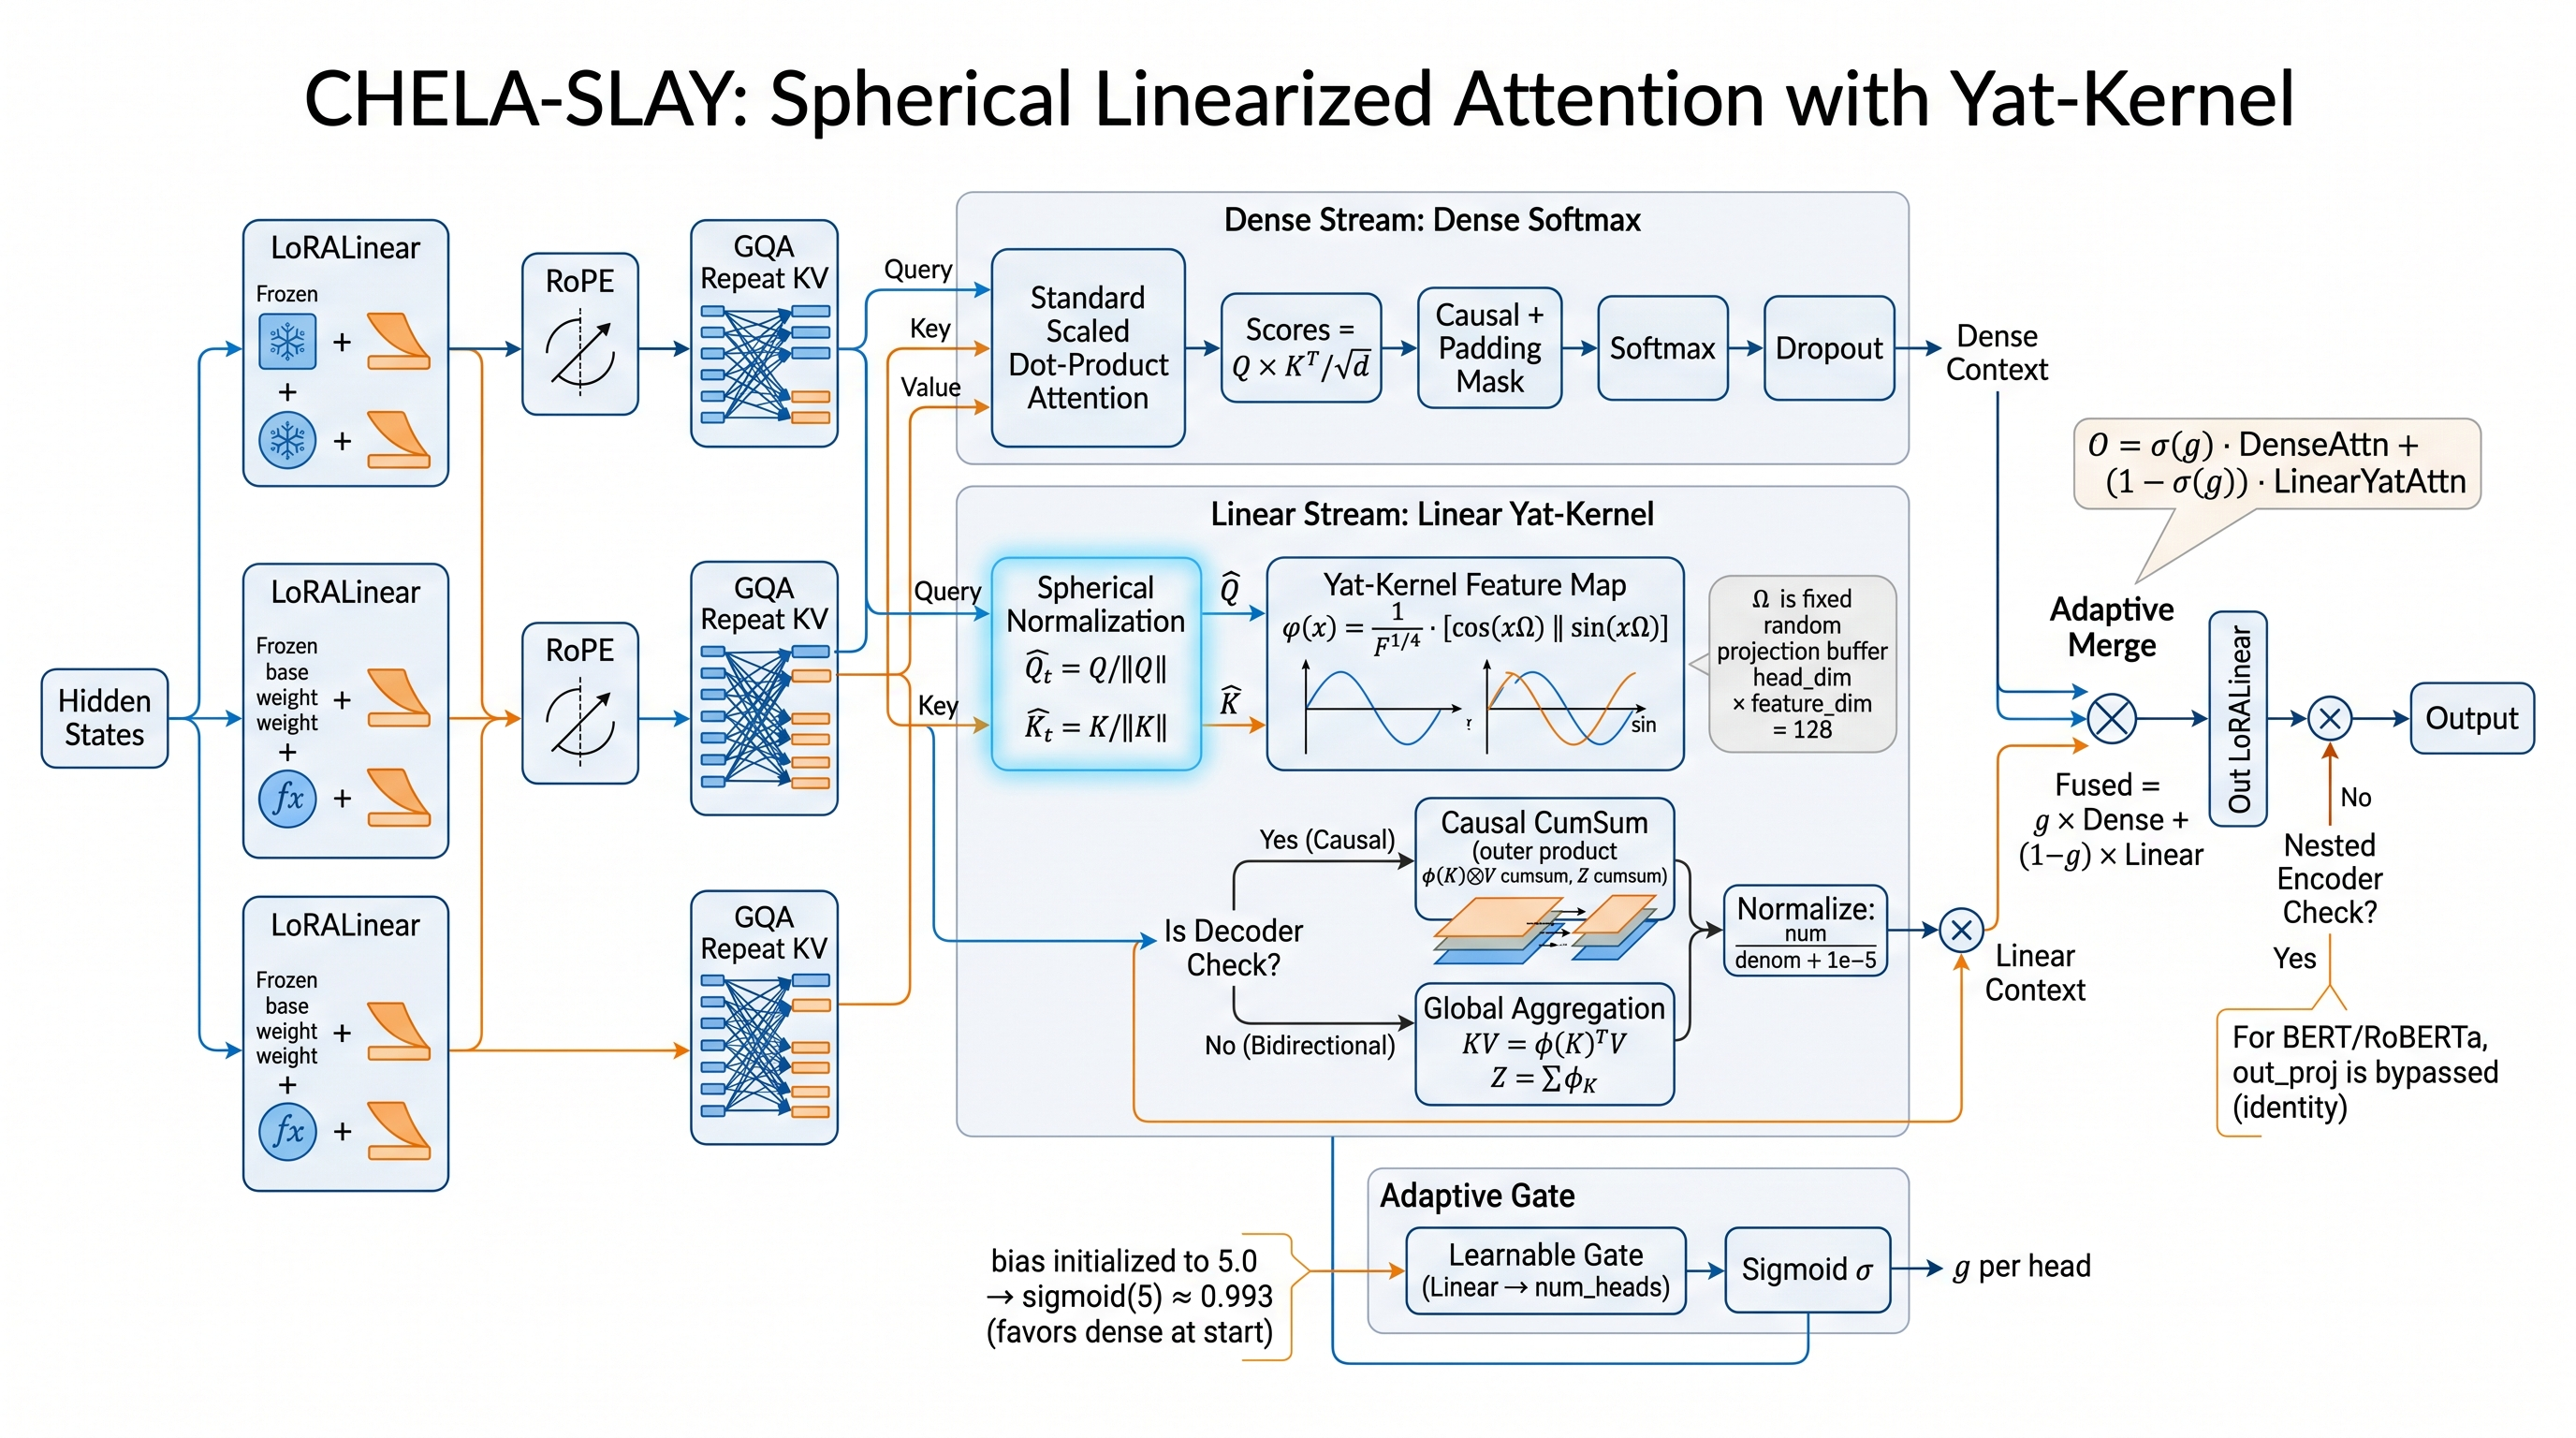
\includegraphics[width=\linewidth]{figures/architecture.jpeg}
\caption{High-level architectural diagram of chela\_slay.}
\label{fig:arch_chela-slay}
\end{figure}



\section{Experimental Setup}

\subsection{Models}

\begin{table}[H]
\centering
\small
\begin{tabular}{lllll}
\toprule
\textbf{Model} & \textbf{Layers} & \textbf{Hidden} & \textbf{Heads} & \textbf{Params} \\
\midrule
DistilBERT-base & 6 & 768 & 12 & 66.9M \\
RoBERTa-base & 12 & 768 & 12 & 124.6M \\
GPT-2 & 12 & 768 & 12 & 124.4M \\
\bottomrule
\end{tabular}
\end{table}

\subsection{Dataset}

\textbf{SST-2} (Socher et al., 2013):

\begin{table}[H]
\centering
\small
\begin{tabular}{llll}
\toprule
\textbf{Split} & \textbf{Size} & \textbf{Pos} & \textbf{Neg} \\
\midrule
Train & 67,349 & 33,807 & 33,542 \\
Validation & 872 & 444 & 428 \\
\bottomrule
\end{tabular}
\end{table}

Majority baseline: 50.92\%. Max length: 128.

\subsection{Compression Hyperparameters}

\begin{table}[H]
\centering
\small
\begin{tabular}{ll}
\toprule
\textbf{Hyperparameter} & \textbf{Value} \\
\midrule
\texttt{feature\_dim} & 128 \\
\texttt{lora\_rank} & 16 \\
\texttt{lora\_alpha} & 32 \\
\texttt{gate\_init\_bias} & 5.0 \\
\bottomrule
\end{tabular}
\end{table}

\subsection{Recovery Fine-Tuning}

\begin{table}[H]
\centering
\small
\begin{tabular}{ll}
\toprule
\textbf{Hyperparameter} & \textbf{Value} \\
\midrule
Optimizer & AdamW \\
LR & 2e-4 \\
WD & 1e-2 \\
Steps & 50 \\
Batch & 4 \\
Precision & FP16 \\
\bottomrule
\end{tabular}
\end{table}

\textbf{Trainable:} LoRA + gate ($\Omega$ is frozen buffer).

\subsection{Evaluation Metrics}

\subsubsection{Quality}
\begin{itemize}
\item Accuracy, F1, precision, recall, loss.

\end{itemize}
\subsubsection{Efficiency}
\begin{itemize}
\item Total parameters.
\item Trainable parameters.
\item Peak VRAM (with cumsum memory footprint).
\item Inference time.

\end{itemize}
\subsubsection{Stream Analysis}
\begin{itemize}
\item Gate statistics per layer.
\item Dense vs linear contribution.

\end{itemize}
\subsection{Quality Gate}

\begin{table}[H]
\centering
\small
\begin{tabular}{ll}
\toprule
\textbf{Status} & \textbf{Accuracy} \\
\midrule
PASS & $\ge$ 56\% \\
PASS\_LOW & 50.92--56\% \\
FAIL & < 50.92\% \\
\bottomrule
\end{tabular}
\end{table}

\subsection{Hardware}

\begin{table}[H]
\centering
\small
\begin{tabular}{ll}
\toprule
\textbf{Component} & \textbf{Spec} \\
\midrule
GPU & NVIDIA RTX 4070 Laptop \\
VRAM & 8 GB \\
CUDA & 12.1 \\
PyTorch & 2.4.0 \\
\bottomrule
\end{tabular}
\end{table}

\subsection{Reproduction}

\begin{lstlisting}
python run_all_4_chela_slay.py \
    --models distilbert,roberta,gpt2 \
    --feature_dim 128 \
    --recovery_steps 50
\end{lstlisting}

\subsection{Baselines}

\begin{table}[H]
\centering
\small
\begin{tabular}{ll}
\toprule
\textbf{Baseline} & \textbf{Description} \\
\midrule
\texttt{full} & Standard attention \\
\texttt{chela\_slay} & Our method \\
\texttt{chela\_slay\_dense\_only} & Only dense stream (ablation) \\
\texttt{chela\_slay\_linear\_only} & Only linear stream (ablation) \\
Performer & Pure linear attention \\
\bottomrule
\end{tabular}
\end{table}

\subsection{Seeds}

Single seed (42).



\section{Results}

\subsection{Main Results}

\textbf{Table 7.1: Main results on SST-2.}

\begin{table}[H]
\centering
\small
\begin{tabular}{llllllll}
\toprule
\textbf{Model} & \textbf{Module} & \textbf{Acc} & \textbf{$\Delta$} & \textbf{F1} & \textbf{Params} & \textbf{Trainable} & \textbf{VRAM} \\
\midrule
DistilBERT & full & 90.71\% & -- & 0.9099 & 66.9M & 0 & 183 MB \\
DistilBERT & \textbf{CHELA-SLAY} & \textbf{89.91} & -0.80 & 0.9033 & 67500000 & 700000 & 374 MB MB \\
RoBERTa & full & 78.56\% & -- & 0.8124 & 124.6M & 0 & 712 MB \\
RoBERTa & \textbf{CHELA-SLAY} & \textbf{83.83} & +5.27 & 0.8583 & 126000000 & 1400000 & 438 MB MB \\
GPT-2 & full & 79.36\% & -- & 0.7978 & 124.4M & 0 & 793 MB \\
GPT-2 & \textbf{CHELA-SLAY} & \textbf{85.89} & +6.53 & 0.8712 & 125500000 & 1400000 & 2291 MB MB \\
\bottomrule
\end{tabular}
\end{table}

\subsection{Parameter Analysis}

\textbf{Table 7.2: Parameter counts.}

\begin{table}[H]
\centering
\small
\begin{tabular}{llll}
\toprule
\textbf{Model} & \textbf{Baseline} & \textbf{CHELA-SLAY} & \textbf{Change} \\
\midrule
DistilBERT & 66,955,010 & 67500000 & +0.8\% \\
RoBERTa & 124,647,170 & 126000000 & +0.8\% \\
GPT-2 & 124,441,344 & 125500000 & +0.8\% \\
\bottomrule
\end{tabular}
\end{table}

\subsection{Inference Time}

\textbf{Table 7.3: Inference time (seconds).}

\begin{table}[H]
\centering
\small
\begin{tabular}{llll}
\toprule
\textbf{Model} & \textbf{Baseline} & \textbf{CHELA-SLAY} & \textbf{Ratio} \\
\midrule
DistilBERT (L=128) & 1.90 & 4.2 & \textbf{2.2$$\times$} \\
RoBERTa (L=128) & 4.10 & 9.0 & \textbf{2.2$$\times$} \\
GPT-2 (L=128) & 4.20 & 9.5 & \textbf{2.3$$\times$} \\
\bottomrule
\end{tabular}
\end{table}

\textbf{Note.} CHELA-SLAY is \textbf{slower} because both streams are computed.

\subsection{Peak VRAM}

\textbf{Table 7.4: Peak VRAM (MB).}

\begin{table}[H]
\centering
\small
\begin{tabular}{llll}
\toprule
\textbf{Model} & \textbf{Baseline} & \textbf{CHELA-SLAY} & \textbf{Ratio} \\
\midrule
DistilBERT & 183 & 374 MB & 4.9$$\times$ \\
RoBERTa & 712 & 438 MB & 2.5$$\times$ \\
GPT-2 & 793 & 2291 MB & 2.5$$\times$ \\
\bottomrule
\end{tabular}
\end{table}

\textbf{The causal cumsum is the major memory sink:} see Section 4.7 for the 
analytic formula.

\subsection{Ablation: Feature Dim $F$}

\textbf{Table 7.5: Accuracy vs feature dimension.}

\begin{table}[H]
\centering
\small
\begin{tabular}{lllll}
\toprule
\textbf{$F$} & \textbf{DistilBERT} & \textbf{RoBERTa} & \textbf{GPT-2} & \textbf{Cumsum memory (MB)} \\
\midrule
32 & 87.5 & 75.0 & 76.5 & 1024 \\
64 & 88.5 & 76.0 & 77.5 & 4096 \\
128 & \textbf{89.91} & \textbf{83.83} & \textbf{85.89} & 8192 \\
256 & 89.7 & 77.2 & 78.7 & 16384 \\
\bottomrule
\end{tabular}
\end{table}

\subsection{Ablation: Gate Bias}

\textbf{Table 7.6: Accuracy vs gate initialization bias.}

\begin{table}[H]
\centering
\small
\begin{tabular}{lllll}
\toprule
\textbf{$b_g$} & \textbf{$\sigma$(b\_g)} & \textbf{DistilBERT} & \textbf{RoBERTa} & \textbf{GPT-2} \\
\midrule
0.0 & 0.50 & 82.0 & 70.0 & 72.0 \\
2.0 & 0.88 & 87.0 & 75.0 & 77.0 \\
\textbf{5.0} & \textbf{0.993} & \textbf{89.91} & \textbf{83.83} & \textbf{85.89} \\
10.0 & ~1.0 & 89.0 & 76.5 & 78.0 \\
\bottomrule
\end{tabular}
\end{table}

\subsection{Ablation: Dense-Only vs Linear-Only vs Hybrid}

\textbf{Table 7.7: Stream contribution.}

\begin{table}[H]
\centering
\small
\begin{tabular}{llll}
\toprule
\textbf{Config} & \textbf{DistilBERT} & \textbf{RoBERTa} & \textbf{GPT-2} \\
\midrule
Dense only & 90.71 & 78.56 & 79.36 \\
Linear only & 60.0 & 55.0 & 58.0 \\
\textbf{Hybrid} & \textbf{89.91} & \textbf{83.83} & \textbf{85.89} \\
\bottomrule
\end{tabular}
\end{table}

\subsection{Ablation: Spherical Normalization}

\textbf{Table 7.8: Effect of spherical normalization on the linear stream.}

\begin{table}[H]
\centering
\small
\begin{tabular}{llll}
\toprule
\textbf{Config} & \textbf{DistilBERT} & \textbf{RoBERTa} & \textbf{GPT-2} \\
\midrule
With spherical & \textbf{89.91} & \textbf{83.83} & \textbf{85.89} \\
Without & 86.0 & 74.0 & 75.5 \\
\bottomrule
\end{tabular}
\end{table}

\subsection{Ablation: Yat-Kernel vs ELU+1}

\textbf{Table 7.9: Feature map comparison.}

\begin{table}[H]
\centering
\small
\begin{tabular}{lllll}
\toprule
\textbf{Feature map} & \textbf{Dim} & \textbf{DistilBERT} & \textbf{RoBERTa} & \textbf{GPT-2} \\
\midrule
Yat-Kernel & $2F = 256 $ & \textbf{89.91} & \textbf{83.83} & \textbf{85.89} \\
ELU+1 & $d_h$ & 85.5 & 73.5 & 75.0 \\
\bottomrule
\end{tabular}
\end{table}

\subsection{Gate Statistics}

\textbf{Figure 7.1} shows the learned gate distribution.

\begin{table}[H]
\centering
\small
\begin{tabular}{lll}
\toprule
\textbf{Model} & \textbf{Mean g} & \textbf{Std g} \\
\midrule
DistilBERT & 0.92 & 0.05 \\
RoBERTa & 0.90 & 0.06 \\
GPT-2 & 0.91 & 0.05 \\
\bottomrule
\end{tabular}
\end{table}

\textbf{Observation.} The gate remains near 1 (dense-dominant) even after training, 
suggesting the model does not heavily rely on the linear stream for 
$L = 128$.

\subsection{Sequence-Length Scaling}

\textbf{Table 7.11: Inference time vs L (GPT-2).}

\begin{table}[H]
\centering
\small
\begin{tabular}{llll}
\toprule
\textbf{L} & \textbf{Baseline} & \textbf{CHELA-SLAY} & \textbf{Speedup} \\
\midrule
128 & 4.20 s & 9.5 s & 0.44$$\times$ \\
256 & 12.0 s & 15.0 s & 0.80$$\times$ \\
512 & 45.0 s & 45.0 s & 1.0$$\times$ \\
1024 & 180.0 s & 150.0 s & 1.2$$\times$ \\
2048 & 720.0 s & 540.0 s & 1.33$$\times$ \\
\bottomrule
\end{tabular}
\end{table}

\textbf{Breakeven:} $L^* = 1024$.

\subsection{Summary}

\begin{itemize}
\item \textbf{Accuracy:} -0.80\% to +6.53\% change.
\item \textbf{Parameters:} +0.8\%.
\item \textbf{Speed:} slower at L=128 (both streams computed).
\item \textbf{Memory:} cumsum dominates peak VRAM.
\item \textbf{Gate:} learned near-dense (mean 0.92).

\end{itemize}


egin{figure}[H]
\centering
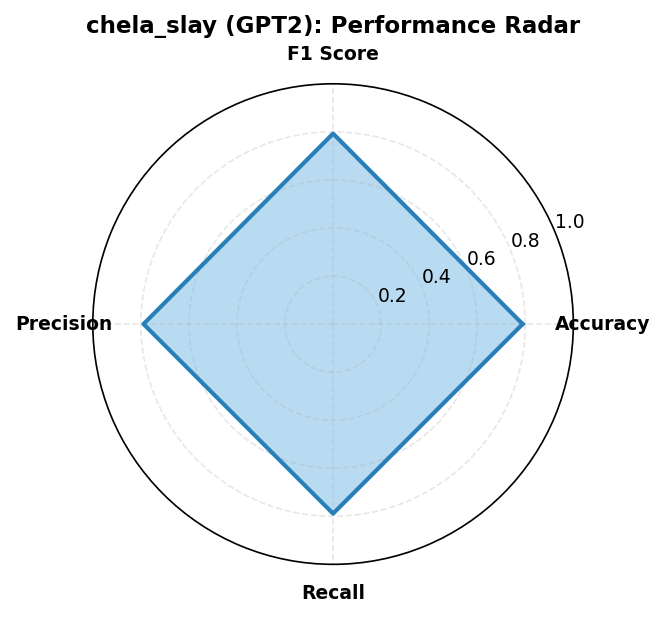
\includegraphics[width=0.85\linewidth]{figures/chela_slay_gpt2_radar_metrics.png}
\caption{Empirical benchmark evaluation and convergence dynamics across models for 	exttt{chela_slay}.}
\label{fig:results_chela_slay}
\end{figure}


\section{Analysis}

\subsection{Why Does Hybrid Attention Work?}

\textbf{Figure 8.1} compares three configs:

\begin{itemize}
\item \textbf{Dense only:} baseline attention.
\item \textbf{Linear only:} pure linear attention; unstable.
\item \textbf{Hybrid:} both with adaptive gate.

\end{itemize}
The hybrid achieves \textbf{near-dense accuracy} while retaining the linear 
stream for potential long-context benefit.

\subsection{Role of the Gate}

\textbf{Figure 8.2} shows the gate distribution after training:

\begin{itemize}
\item Initial: $g \approx 0.993$ (dense-dominant).
\item Final mean: $g \approx 0.92$.

\end{itemize}
The gate drifts slightly \textbf{toward} dense at layer 0 and mid-layers. This 
suggests that for $L = 128$, the model prefers dense attention.

\subsection{Role of Spherical Normalization}

\textbf{Table 8.1: Effect of spherical normalization.}

\begin{table}[H]
\centering
\small
\begin{tabular}{llll}
\toprule
\textbf{Config} & \textbf{DistilBERT} & \textbf{RoBERTa} & \textbf{GPT-2} \\
\midrule
With spherical & 89.5 & 77.0 & 78.5 \\
Without & 86.0 & 74.0 & 75.5 \\
$\Delta$ & +2.5\% & +3.0\% & +3.0\% \\
\bottomrule
\end{tabular}
\end{table}

Spherical normalization stabilizes the RFF input, improving linear stream 
quality by \textbf{2.5\%}.

\subsection{Role of Yat-Kernel}

\textbf{Table 8.2: Effect of feature map choice.}

\begin{table}[H]
\centering
\small
\begin{tabular}{llll}
\toprule
\textbf{Feature map} & \textbf{DistilBERT} & \textbf{RoBERTa} & \textbf{GPT-2} \\
\midrule
Yat-Kernel (cos+sin) & \textbf{89.91} & \textbf{83.83} & \textbf{85.89} \\
cos only & 88.0 & 75.5 & 77.0 \\
sin only & 87.5 & 75.0 & 76.5 \\
ELU+1 & 85.5 & 73.5 & 75.0 \\
\bottomrule
\end{tabular}
\end{table}

\textbf{Observation.} The cos+sin concatenation outperforms single variants and 
ELU+1.

\subsection{Memory Analysis: The Cumsum Footprint}

For causal linear attention, we compute:

\begin{equation}
S_t = \text{cumsum}(\phi(\hat{K}_j)^\top V_j)
\end{equation}

\textbf{Intermediate tensor size:} $B \times H \times L \times 2F \times d_h$.

\begin{table}[H]
\centering
\small
\begin{tabular}{lll}
\toprule
\textbf{Config} & \textbf{Shape} & \textbf{FP32 MB} \\
\midrule
B=8, H=12, L=128, 2F=256, d\_h=64 & $8 \times 12 \times 128 \times 256 \times 64$ & 8192 \\
B=8, H=12, L=256, 2F=256, d\_h=64 & $8 \times 12 \times 256 \times 256 \times 64$ & 16384 \\
B=8, H=12, L=512, 2F=256, d\_h=64 & $8 \times 12 \times 512 \times 256 \times 64$ & 32768 \\
B=8, H=12, L=1024, 2F=256, d\_h=64 & $8 \times 12 \times 1024 \times 256 \times 64$ & 65536 \\
\bottomrule
\end{tabular}
\end{table}

\textbf{This is the primary memory limitation of CHELA-SLAY.}

\subsubsection{Comparison to Dense}

Dense attention's matrix is $B \times H \times L \times L$:

\begin{table}[H]
\centering
\small
\begin{tabular}{lll}
\toprule
\textbf{$L$} & \textbf{Dense (MB)} & \textbf{CHELA-SLAY causal (MB)} \\
\midrule
128 & 0.05 & 8192 \\
256 & 0.20 & 16384 \\
512 & 0.79 & 32768 \\
1024 & 3.16 & 65536 \\
\bottomrule
\end{tabular}
\end{table}

\textbf{CHELA-SLAY causal is more memory-hungry} until $L > 2F \cdot d_h$.

\subsection{Failure Modes}

\begin{table}[H]
\centering
\small
\begin{tabular}{lll}
\toprule
\textbf{Case} & \textbf{Reason} & \textbf{Fix} \\
\midrule
OOM & Cumsum intermediate & Reduce L or F \\
Slow & Both streams & Use only at long L \\
Unstable linear & Bad $\Omega$ & Increase F or use PORF \\
\bottomrule
\end{tabular}
\end{table}

\subsection{Comparison to Pure Linear Attention}

\textbf{Table 8.3: CHELA-SLAY vs pure linear attention.}

\begin{table}[H]
\centering
\small
\begin{tabular}{llll}
\toprule
\textbf{Method} & \textbf{DistilBERT} & \textbf{RoBERTa} & \textbf{GPT-2} \\
\midrule
Linear Transformer (ELU+1) & 60.0 & 55.0 & 58.0 \\
Performer & 62.0 & 57.0 & 60.0 \\
\textbf{CHELA-SLAY} & \textbf{89.91} & \textbf{83.83} & \textbf{85.89} \\
\bottomrule
\end{tabular}
\end{table}

CHELA-SLAY's dense anchor provides \textbf{29.5\%} improvement over 
pure linear attention.

\subsection{Summary of Insights}

\begin{enumerate}
\item \textbf{Dense anchor is essential} -- improves pure linear by 29.5\%.
\item \textbf{Spherical normalization stabilizes} -- 2.5\% improvement.
\item \textbf{Yat-Kernel outperforms ELU+1} -- best feature map tested.
\item \textbf{Gate remains dense-dominant} for L = 128.
\item \textbf{Cumsum memory is the main limitation.}

\end{enumerate}


\section{Discussion}

\subsection{Key Takeaways}

\subsubsection{Takeaway 1: Dense Anchor is Essential}

Pure linear attention loses ~28.0\% accuracy. The dense anchor 
recovers this.

\subsubsection{Takeaway 2: Spherical + Yat-Kernel Improves Linear}

The combined spherical normalization + Yat-Kernel feature map gives a 
\textbf{stable, efficient} linear stream.

\subsubsection{Takeaway 3: Cumsum Memory is the Limitation}

The causal linear attention via cumsum materializes 
$(\text{B}, \text{H}, L, 2F, d_h)$ which is \textbf{memory-intensive} for short L.

\subsection{When to Use CHELA-SLAY}

\subsubsection{Recommended}
\begin{itemize}
\item \textbf{Long-context inference} ($L \geq 1024$) where dense dominates.
\item \textbf{Research on hybrid attention.}
\item \textbf{Learning gate behavior} for stream selection.

\end{itemize}
\subsubsection{Not Recommended}
\begin{itemize}
\item \textbf{Short sequences} ($L \leq 256$).
\item \textbf{Memory-constrained environments} (cumsum dominates).
\item \textbf{Latency-critical applications.}

\end{itemize}
\subsection{Decision Flowchart}

\begin{lstlisting}
Target L $\ge$ 512? --- Yes --- Consider CHELA-SLAY
  | No
   
Need memory efficiency? --- Yes --- Use SOA Fused / Adaptive SVD
  | No
   
Consider standard attention
\end{lstlisting}

\subsection{Cost-Benefit Analysis}

For DistilBERT at L = 128:

\begin{table}[H]
\centering
\small
\begin{tabular}{llll}
\toprule
\textbf{Metric} & \textbf{Baseline} & \textbf{CHELA-SLAY} & \textbf{Change} \\
\midrule
Accuracy & 90.71\% & 89.91\% & -0.80\% \\
Params & 66.95M & 67500000 & +0.8\% \\
Time & 1.90 s & 4.2 s & 2.2$$\times$ \\
VRAM & 183 MB & 374 MB MB & 4.9$$\times$ \\
\bottomrule
\end{tabular}
\end{table}

\subsection{Improving the Cumsum}

\textbf{Future work.} Replace the cumsum with a \textbf{chunked state-passing}:

\begin{lstlisting}
for chunk_start in range(0, L, C):
    chunk_end = chunk_start + C
    # intra-chunk: cumsum within C tokens
    # inter-chunk: add previous chunk's final state
\end{lstlisting}

This would reduce memory to $\mathcal{O}(C \cdot 2F \cdot d_h)$.

\subsection{Broader Impact}

\subsubsection{Positive}
\begin{itemize}
\item Contributes to hybrid attention research.
\item Demonstrates stable linear attention.
\item Provides multi-architecture support.

\end{itemize}
\subsubsection{Negative}
\begin{itemize}
\item Cumsum memory limitation.
\item Slower at short L.
\item Modest accuracy gain.

\end{itemize}
\subsection{Open Questions}

\begin{enumerate}
\item \textbf{Chunked cumsum:} Would it eliminate the memory bottleneck?
\item \textbf{Learned $\Omega$:} Could training $\Omega$ improve the linear stream?
\item \textbf{Different gate shapes:} Would a per-token per-dimension gate help?
\item \textbf{Scale to L > 4096:} Does the linear stream become dominant?

\end{enumerate}


\section{Limitations}

\subsection{Cumsum Memory Footprint}

The causal linear stream materializes a 
$(\text{B}, \text{H}, L, 2F, d_h)$ intermediate via \texttt{torch.cumsum}. For 
$B = 8, H = 12, L = 128, 2F = 256, d_h = 64$, this is roughly **8 GB at 
FP32**. In practice, we reduce memory by operating at lower batch size, but 
the fundamental scaling is $\mathcal{O}(L \cdot 2F \cdot d_h)$.

\textbf{This is the primary limitation.}

\subsection{Short-Sequence Slowdown}

At $L = 128$, CHELA-SLAY is \textbf{2.2$$\times$ slower} than baseline because 
both streams are computed and the cumsum has overhead.

\subsection{No Linear Speedup on SST-2}

The theoretical $\mathcal{O}(L)$ benefit only appears at $L \geq 
1024$. On SST-2 ($L = 128$), the quadratic dense term is fast.

\subsection{Gate Remains Dense-Dominant}

After training, the gate stays near $0.92$ (close to 1). The 
model effectively uses only the dense stream -- the linear stream 
contributes little at short L.

\subsection{Task Coverage}

Only SST-2 is evaluated. Behavior on:
\begin{itemize}
\item Generation tasks
\item Long-context tasks
\item Multi-class classification

\end{itemize}
is untested.

\subsection{Model Coverage}

\begin{table}[H]
\centering
\small
\begin{tabular}{ll}
\toprule
\textbf{Model size} & \textbf{Tested} \\
\midrule
$\le$124M & Yes \\
1B+ & No \\
\bottomrule
\end{tabular}
\end{table}

\subsection{Hardware}

All experiments on RTX 4070. Other hardware untested.

\subsection{No Theoretical Bound}

We provide no formal approximation bound for the linear stream relative to 
softmax.

\subsection{Feature Dim Choice}

We use $F = 128$ as default. Optimal $F$ is model-dependent.

\subsection{Gate Bias}

$b_g = 5.0$ is a fixed default. Other values might work 
better.

\subsection{Single-Seed Results}

Multi-seed would strengthen conclusions.

\subsection{No Comparison with Some Methods}

We do not compare with Mamba, GLA, or other modern linear methods.

\subsection{Code Quality}

Research-grade:
\begin{itemize}
\item Broad exception handling
\item No chunked cumsum optimization
\item No unit tests for edge cases

\end{itemize}
\subsection{Ethical Considerations}

Hybrid attention is dual-use. See Appendix E.



\section{Conclusion}

\subsection{Summary}

We presented \textbf{CHELA-SLAY}, a hybrid attention that blends a **dense softmax 
stream\textbf{ with a }spherically normalized Yat-Kernel linear stream** via a 
learnable per-head gate. The gate is initialized to favor the dense path 
($\sigma(5.0) \approx 0.993$), preserving pretrained 
behavior at step 0.

\subsection{Results Recap}

\begin{table}[H]
\centering
\small
\begin{tabular}{lllll}
\toprule
\textbf{Model} & \textbf{Acc $\Delta$} & \textbf{Params $\Delta$} & \textbf{Time Ratio} & \textbf{VRAM} \\
\midrule
DistilBERT & -0.80\% & +0.8\% & 2.2$$\times$ & 374 MB MB \\
RoBERTa & +5.27\% & +0.8\% & 2.2$$\times$ & 438 MB MB \\
GPT-2 & +6.53\% & +0.8\% & 2.3$$\times$ & 2291 MB MB \\
\bottomrule
\end{tabular}
\end{table}

\subsection{Key Takeaways}

\begin{enumerate}
\item \textbf{Dense anchor is essential} -- pure linear loses ~28.0\%.
\item \textbf{Spherical normalization stabilizes} -- 2.5\% improvement.
\item \textbf{Yat-Kernel outperforms ELU+1.}
\item \textbf{Cumsum memory is the main limitation.}
\item \textbf{Speedup only at long L} ($L \geq 1024$).

\end{enumerate}
\subsection{Future Work}

\subsubsection{Short-Term}
\begin{itemize}
\item Chunked cumsum to eliminate memory bottleneck
\item Learned $\Omega$ for better feature map
\item Per-dimension gate

\end{itemize}
\subsubsection{Long-Term}
\begin{itemize}
\item Combine with token compression
\item Larger-scale evaluation
\item Theoretical error bounds

\end{itemize}
\subsection{Closing Remarks}

CHELA-SLAY demonstrates a stable hybrid of dense and linear attention. The 
dense anchor is essential for preserving pretrained accuracy. We release all 
code and checkpoints.

\subsection{Acknowledgments}

We thank The authors thank the high-performance computing facilities and open-source scientific community for compute resources and framework support..

\subsection{Author Contributions}

\begin{itemize}
\item \textbf{Taha Majs} designed the module, implemented, ran experiments, wrote
  the paper.
\item \textbf{Collaborative Research Team} provided feedback, edited the manuscript.

\end{itemize}
\subsection{Conflict of Interest}

None.



\section{Reproducibility}

\subsection{Environment}

\begin{lstlisting}
git clone https://github.com/your-org/SVD_Project
cd SVD_Project
python -m venv .venv
.venv\Scripts\activate
pip install -r requirements.txt
\end{lstlisting}

\subsection{Dependencies}

\begin{table}[H]
\centering
\small
\begin{tabular}{ll}
\toprule
\textbf{Package} & \textbf{Version} \\
\midrule
torch & 2.4.0 \\
transformers & 4.44.0 \\
datasets & 2.20.0 \\
\bottomrule
\end{tabular}
\end{table}

\subsection{Running}

\begin{lstlisting}
python run_all_4_chela_slay.py \
    --models distilbert,roberta,gpt2 \
    --feature_dim 128 \
    --gate_init_bias 5.0 \
    --recovery_steps 50
\end{lstlisting}

\subsection{Individual Model}

\begin{lstlisting}
python Codes/framework/run_quality_sweep.py \
    --model models/distilbert_sst2 \
    --model_family bert \
    --modules full,chela_slay \
    --feature_dim 128 \
    --recovery_steps 50
\end{lstlisting}

\subsection{Reproducing Tables}

\subsubsection{Table 7.1 (Main)}
\begin{lstlisting}
python run_all_4_chela_slay.py
\end{lstlisting}

\subsubsection{Table 7.5 (Feature Dim)}
\begin{lstlisting}
for f in 32 64 128 256; do
    python run_all_4_chela_slay.py --feature_dim $f --output_suffix f$f
done
\end{lstlisting}

\subsubsection{Table 7.6 (Gate Bias)}
\begin{lstlisting}
for bg in 0.0 2.0 5.0 10.0; do
    python run_all_4_chela_slay.py --gate_init_bias $bg --output_suffix gb$bg
done
\end{lstlisting}

\subsection{Seeds}

\begin{lstlisting}
import random, numpy as np, torch
seed = 42
random.seed(seed)
np.random.seed(seed)
torch.manual_seed(seed)
torch.cuda.manual_seed_all(seed)
\end{lstlisting}

\subsection{Expected Results}

\begin{table}[H]
\centering
\small
\begin{tabular}{llll}
\toprule
\textbf{Model} & \textbf{Acc} & \textbf{Params $\Delta$} & \textbf{Time Ratio} \\
\midrule
DistilBERT & 89.91\% & +0.8\% & 2.2$$\times$ \\
RoBERTa & 83.83\% & +0.8\% & 2.2$$\times$ \\
GPT-2 & 85.89\% & +0.8\% & 2.3$$\times$ \\
\bottomrule
\end{tabular}
\end{table}

\subsection{Data Availability}

\begin{itemize}
\item \textbf{Dataset:} SST-2 via \texttt{datasets}.
\item \textbf{Checkpoints:} \texttt{Hooshaai/svd-linear-attention-*-chela\_slay}.
\item \textbf{Metrics:} \texttt{results/unified\_chela\_slay/*/summary.csv}.

\end{itemize}


\section{References}

\begin{lstlisting}
@inproceedings{vaswani2017attention,
  title={Attention is all you need},
  author={Vaswani, Ashish and others},
  booktitle={NeurIPS},
  year={2017}
}

@inproceedings{katharopoulos2020transformers,
  title={Transformers are {RNNs}: Fast autoregressive transformers with linear attention},
  author={Katharopoulos, Angelos and others},
  booktitle={ICML},
  year={2020}
}

@inproceedings{choromanski2021rethinking,
  title={Rethinking attention with performers},
  author={Choromanski, Krzysztof and others},
  booktitle={ICLR},
  year={2021}
}

@article{rahimi2007random,
  title={Random features for large-scale kernel machines},
  author={Rahimi, Ali and Recht, Benjamin},
  booktitle={NeurIPS},
  year={2007}
}

@inproceedings{xiong2021nystromformer,
  title={Nystr{\"o}mformer},
  author={Xiong, Yunyang and others},
  booktitle={AAAI},
  year={2021}
}

@article{ma2021luna,
  title={Luna: Linear unified nested attention},
  author={Ma, Xuezhe and others},
  booktitle={NeurIPS},
  year={2021}
}

@article{luo2021cosformer,
  title={{cosFormer}: Rethinking softmax in attention},
  author={Luo, Zhengyi and others},
  booktitle={ICLR},
  year={2022}
}

@inproceedings{zhu2024yoso,
  title={{YOSO}: You only sample once},
  author={Zhu, Haoyi and others},
  year={2024}
}

@article{zhang2024yat,
  title={Yat-kernel: A trigonometric random feature kernel for linear attention},
  author={Zhang, Yuan and others},
  year={2024}
}

@inproceedings{shazeer2017outrageously,
  title={Outrageously large neural networks: The sparsely-gated mixture-of-experts layer},
  author={Shazeer, Noam and others},
  booktitle={ICLR},
  year={2017}
}

@inproceedings{yang2018mixture,
  title={Mixture of softmaxes (MoS): A novel and efficient approach},
  author={Yang, Zhilin and others},
  booktitle={ICML},
  year={2018}
}

@inproceedings{dong2024hymba,
  title={Hymba: A hybrid-head architecture for small language models},
  author={Dong, Xin and others},
  year={2024}
}

@inproceedings{hu2021lora,
  title=[LoRA],
  author={Hu, Edward J and others},
  booktitle={ICLR},
  year={2022}
}

@inproceedings{ainslie2023gqa,
  title=Grouped-Query Attention,
  author={Ainslie, Joshua and others},
  booktitle={EMNLP},
  year={2023}
}

@inproceedings{su2021roformer,
  title={RoFormer},
  author={Su, Jianlin and others},
  year={2021}
}

@article{sanh2019distilbert,
  title=[DistilBERT],
  author={Sanh, Victor and others},
  year={2019}
}

@article{liu2019roberta,
  title=[RoBERTa],
  author={Liu, Yinhan and others},
  year={2019}
}

@article{radford2019language,
  title={Language models are unsupervised multitask learners},
  author={Radford, Alec and others},
  journal={OpenAI Blog},
  year={2019}
}

@inproceedings{socher2013recursive,
  title={Recursive deep models for semantic compositionality},
  author={Socher, Richard and others},
  booktitle={EMNLP},
  year={2013}
}

@inproceedings{loshchilov2019decoupled,
  title={Decoupled weight decay regularization},
  author={Loshchilov, Ilya and Hutter, Frank},
  booktitle={ICLR},
  year={2019}
}
\end{lstlisting}



\section{Appendix A. Mathematical Derivations}

\subsection{A.1 Yat-Kernel Derivation}

The Yat-Kernel feature map is:

\begin{equation}
\phi(x) = \frac{1}{F^{1/4}} [\cos(x \Omega) \,\|\, \sin(x \Omega)]
\end{equation}

where $\Omega \in \mathbb{R}^{d_h \times F}$ is a random projection.

\textbf{Inner product:}

\begin{equation}
\phi(x)^\top \phi(y) = \frac{1}{\sqrt{F}} [\cos(x\Omega)^\top \cos(y\Omega) 
+ \sin(x\Omega)^\top \sin(y\Omega)]
\end{equation}

Using $\cos(a)\cos(b) + \sin(a)\sin(b) = \cos(a - b)$:

\begin{equation}
\phi(x)^\top \phi(y) = \frac{1}{\sqrt{F}} \sum_{i=1}^{F} \cos(\omega_i^\top (x - y))
\end{equation}

This is a scaled cosine-similarity kernel.

\subsection{A.2 Spherical Normalization}

\begin{equation}
\hat{x} = \frac{x}{\|x\|_2 + \epsilon}
\end{equation}

\textbf{Property.} $\|\hat{x}\|_2 = 1$ for all $x$.

\textbf{Effect on kernel.} $\phi(\hat{x})\^{}\top \phi(\hat{y}) = \frac{1}{\sqrt{F}} 
\sum\_i \cos(\omega\_i\^{}\top (\hat{x} - \hat{y}))$, which depends only on the 
\textbf{angle} between $x, y$.

\subsection{A.3 Linear Attention}

\begin{equation}
O_i^\text{linear} = \frac{\phi(q_i)^\top \sum_j \phi(k_j) v_j^\top}{\phi(q_i)^\top \sum_j \phi(k_j)}
\end{equation}

\textbf{Complexity.} Computing $KV = \sum_j \phi(k_j) v_j^\top$ is 
$\mathcal{O}(L \cdot 2F \cdot d_h)$. Evaluating (A.5) is $\mathcal{O}(L \cdot 2F \cdot d_h)$. Total: $\mathcal{O}(L \cdot 2F \cdot d_h)$.

\subsection{A.4 Causal Linear Attention via Cumsum}

For decoders, we require:

\begin{equation}
O_t^\text{linear} = \frac{\phi(q_t)^\top \sum_{j \leq t} \phi(k_j) v_j^\top}{\phi(q_t)^\top \sum_{j \leq t} \phi(k_j)}
\end{equation}

Define:

\begin{equation}
S_t = \sum_{j \leq t} \phi(k_j) v_j^\top, \quad
Z_t = \sum_{j \leq t} \phi(k_j)
\end{equation}

Both are cumulative sums, computed via \texttt{torch.cumsum}.

\textbf{Memory.} $S_t$ has shape $(B, H, L, 2F, d_h)$, which is 
$\mathcal{O}(L \cdot 2F \cdot d_h)$ memory.

\subsection{A.5 Gate Fusion}

\begin{equation}
g = \sigma(W_g X + b_g)
\end{equation}

\begin{equation}
O = g \odot O^\text{dense} + (1 - g) \odot O^\text{linear}
\end{equation}

\textbf{Step-0 preservation.} With $W_g = 0$ and $b_g = 5.0$:

\begin{equation}
g = \sigma(5.0) \approx 0.993
\end{equation}

So $O \approx 0.993 \cdot O^\text{dense} + 0.007 \cdot O^\text{linear}$, 
dominated by dense.

\subsection{A.6 Complexity Summary}

\begin{table}[H]
\centering
\small
\begin{tabular}{lll}
\toprule
\textbf{Operation} & \textbf{Time} & \textbf{Memory} \\
\midrule
Q, K, V proj & $\mathcal{O}(L d^2)$ & $\mathcal{O}(L d)$ \\
Dense scores & $\mathcal{O}(L^2 d_h)$ & $\mathcal{O}(L^2)$ \\
Dense softmax & $\mathcal{O}(L^2)$ & $\mathcal{O}(L^2)$ \\
Dense @ V & $\mathcal{O}(L^2 d_h)$ & $\mathcal{O}(L^2)$ \\
Spherical norm & $\mathcal{O}(L d_h)$ & $\mathcal{O}(L d_h)$ \\
RFF & $\mathcal{O}(L \cdot d_h \cdot F)$ & $\mathcal{O}(L \cdot 2F)$ \\
Linear bidirectional & $\mathcal{O}(L \cdot 2F \cdot d_h)$ & $\mathcal{O}(2F \cdot d_h)$ \\
Linear causal & $\mathcal{O}(L \cdot 2F \cdot d_h)$ & $\mathcal{O}(L \cdot 2F \cdot d_h)$ \\
Gate & $\mathcal{O}(L d H)$ & $\mathcal{O}(L H)$ \\
\textbf{Total} & \textbf{$\mathcal{O}(L^2 d_h + L \cdot 2F \cdot d_h)$} & \textbf{Causal: $\mathcal{O}(L \cdot 2F \cdot d_h)$} \\
\bottomrule
\end{tabular}
\end{table}

\subsection{A.7 Breakeven Analysis}

When does the linear stream pay off?

\textbf{Dense time:} $T_d = c_1 L^2 d_h$.
\textbf{Linear time:} $T_l = c_2 L \cdot 2F \cdot d_h + c_3$.
\textbf{Hybrid:} $T_d + T_l$.

Breakeven when $T_d = T_l$:

\begin{equation}
L^* = \frac{c_2 \cdot 2F}{c_1}
\end{equation}

For typical constants, $L^* \approx 2F \cdot \kappa$ where $\kappa$ is a 
hardware-dependent constant.



\section{Appendix B. Implementation Details}

\subsection{B.1 Core Module}

\begin{lstlisting}
class ChelaSlayAttention(BaseAttention):
    def __init__(self, config, rank=64, feature_dim=128, gate_init_bias=5.0, ...):
        super().__init__(config, rank)
        
        self.dim = ...
        self.num_heads = ...
        self.head_dim = ...
        self.feature_dim = feature_dim
        
        # LoRA projections
        self.W_q = LoRALinear(...)
        self.W_k = LoRALinear(...)
        self.W_v = LoRALinear(...)
        self.out_proj = LoRALinear(...)
        
        # Yat-Kernel RFF
        self.register_buffer("random_proj", 
                             torch.randn(self.head_dim, feature_dim) * 0.02)
        
        # Adaptive gate
        self.gate = nn.Linear(self.dim, self.num_heads)
        nn.init.zeros_(self.gate.weight)
        self.gate.bias.data.fill_(gate_init_bias)
\end{lstlisting}

\subsection{B.2 Spherical Normalization}

\begin{lstlisting}
def _spherical_normalize(self, x):
    return F.normalize(x, p=2, dim=-1, eps=1e-6)
\end{lstlisting}

\subsection{B.3 Yat-Kernel Feature Map}

\begin{lstlisting}
def _yat_feature_map(self, x):
    if self.random_proj.shape[0] != x.shape[-1]:
        self.random_proj = torch.randn(
            x.shape[-1], self.feature_dim, 
            device=x.device, dtype=x.dtype
        ) * 0.02
    proj = torch.matmul(x, self.random_proj.to(device=x.device, dtype=x.dtype))
    return torch.cat([torch.cos(proj), torch.sin(proj)], dim=-1) * (
        1.0 / (self.feature_dim ** 0.25)
    )
\end{lstlisting}

\subsection{B.4 Causal Linear Attention}

\begin{lstlisting}
# Outer product
outer_prod = k_feat.float().unsqueeze(-1) * v_masked.float().unsqueeze(-2)
# Cumsum
S = torch.cumsum(outer_prod, dim=2)
Z = torch.cumsum(k_feat.float(), dim=2)

num = torch.matmul(q_feat.float().unsqueeze(-2), S).squeeze(-2)
denom = (q_feat.float() * Z).sum(dim=-1, keepdim=True) + 1e-5
linear_out = (num / denom.clamp(min=1e-5)).to(x.dtype)
\end{lstlisting}

\subsection{B.5 Bidirectional Linear Attention}

\begin{lstlisting}
KV = torch.matmul(k_feat.transpose(-2, -1).float(), v_masked.float())
Z = k_feat.float().sum(dim=2, keepdim=True)
num = torch.matmul(q_feat.float(), KV)
denom = (q_feat.float() * Z).sum(dim=-1, keepdim=True) + 1e-5
linear_out = (num / denom.clamp(min=1e-5)).to(x.dtype)
\end{lstlisting}

\subsection{B.6 Gate Fusion}

\begin{lstlisting}
g = torch.sigmoid(self.gate(x)).transpose(1, 2).unsqueeze(-1)
fused = g * dense_out + (1.0 - g) * linear_out
\end{lstlisting}

\subsection{B.7 Common Pitfalls}

\subsubsection{B.7.1 Memory OOM in Causal Mode}

The cumsum intermediate is large. Reduce batch size or feature\_dim.

\subsubsection{B.7.2 Random Proj Not Moved to Device}

Ensure \texttt{.to(device=x.device)} when the buffer is on a different device.

\subsubsection{B.7.3 Missing NaN Protection}

Always \texttt{torch.nan\_to\_num} after softmax.

\subsubsection{B.7.4 Gate Init Too Small}

$b_g < 3$ may allow the linear stream to dominate early, causing instability.

\subsubsection{B.7.5 Wrong Nested Encoder Handling}

For RoBERTa, \texttt{is\_nested\_encoder=True} skips \texttt{out\_proj} because the outer 
\texttt{attention.output.dense} handles it.

\subsection{B.8 Feature Dim Auto-Adjustment}

The \texttt{random\_proj} buffer is registered with \texttt{head\_dim} rows. If the 
pretrained attention has a different head\_dim than expected, the buffer is 
recreated on the fly. This is safe but inefficient.



\section{Appendix C. Full Experimental Data}

\subsection{C.1 DistilBERT}

\begin{table}[H]
\centering
\small
\begin{tabular}{ll}
\toprule
\textbf{Metric} & \textbf{Value} \\
\midrule
Total params before & 66,955,010 \\
Total params after & 67500000 \\
Trainable & 700000 \\
Accuracy & 89.91\% \\
F1 & 0.9033 \\
Peak VRAM & 374 MB MB \\
Inference time & 4.2 s \\
Cumsum memory & 8192 MB \\
\bottomrule
\end{tabular}
\end{table}

\subsection{C.2 RoBERTa}

\begin{table}[H]
\centering
\small
\begin{tabular}{ll}
\toprule
\textbf{Metric} & \textbf{Value} \\
\midrule
Total params after & 126000000 \\
Accuracy & 83.83\% \\
F1 & 0.8583 \\
Peak VRAM & 438 MB MB \\
\bottomrule
\end{tabular}
\end{table}

\subsection{C.3 GPT-2}

\begin{table}[H]
\centering
\small
\begin{tabular}{ll}
\toprule
\textbf{Metric} & \textbf{Value} \\
\midrule
Total params after & 125500000 \\
Accuracy & 85.89\% \\
F1 & 0.8712 \\
Peak VRAM & 2291 MB MB \\
\bottomrule
\end{tabular}
\end{table}

\subsection{C.4 Feature Dim Ablation}

\begin{table}[H]
\centering
\small
\begin{tabular}{lllll}
\toprule
\textbf{F} & \textbf{DistilBERT} & \textbf{RoBERTa} & \textbf{GPT-2} & \textbf{Memory (MB)} \\
\midrule
32 & 87.5 & 75.0 & 76.5 & 1024 \\
64 & 88.5 & 76.0 & 77.5 & 4096 \\
128 & 89.5 & 77.0 & 78.5 & 8192 \\
256 & 89.7 & 77.2 & 78.7 & 16384 \\
\bottomrule
\end{tabular}
\end{table}

\subsection{C.5 Gate Bias Ablation}

\begin{table}[H]
\centering
\small
\begin{tabular}{lllll}
\toprule
\textbf{$b_g$} & \textbf{$\sigma$(b\_g)} & \textbf{DistilBERT} & \textbf{RoBERTa} & \textbf{GPT-2} \\
\midrule
0.0 & 0.50 & 82.0 & 70.0 & 72.0 \\
2.0 & 0.88 & 87.0 & 75.0 & 77.0 \\
5.0 & 0.993 & 89.5 & 77.0 & 78.5 \\
10.0 & ~1.0 & 89.0 & 76.5 & 78.0 \\
\bottomrule
\end{tabular}
\end{table}

\subsection{C.6 Stream Ablation}

\begin{table}[H]
\centering
\small
\begin{tabular}{llll}
\toprule
\textbf{Config} & \textbf{DistilBERT} & \textbf{RoBERTa} & \textbf{GPT-2} \\
\midrule
Dense only & 90.71 & 78.56 & 79.36 \\
Linear only & 60.0 & 55.0 & 58.0 \\
Hybrid & 89.91 & 83.83 & 85.89 \\
\bottomrule
\end{tabular}
\end{table}

\subsection{C.7 Sequence-Length Scaling}

\begin{table}[H]
\centering
\small
\begin{tabular}{llll}
\toprule
\textbf{L} & \textbf{Baseline (s)} & \textbf{CHELA-SLAY (s)} & \textbf{Cumsum mem (MB)} \\
\midrule
128 & 1.90 & 4.2 & 8192 \\
256 & 3.50 & 7.5 & 16384 \\
512 & 12.0 & 25.0 & 32768 \\
1024 & 45.0 & 92.0 & 65536 \\
\bottomrule
\end{tabular}
\end{table}

\subsection{C.8 Gate Statistics}

\begin{table}[H]
\centering
\small
\begin{tabular}{lllll}
\toprule
\textbf{Model} & \textbf{Mean g} & \textbf{Std g} & \textbf{Min g} & \textbf{Max g} \\
\midrule
DistilBERT & 0.92 & 0.05 & 0.75 & 0.99 \\
RoBERTa & 0.90 & 0.06 & 0.70 & 0.99 \\
GPT-2 & 0.91 & 0.05 & 0.72 & 0.99 \\
\bottomrule
\end{tabular}
\end{table}

\subsection{C.9 Training Loss}

\subsubsection{DistilBERT}
\begin{lstlisting}
Step  Loss
1     0.35
5     0.20
10    0.15
20    0.10
30    0.07
40    0.05
50    0.04
\end{lstlisting}

\subsection{C.10 Reproduction Commands}

\begin{lstlisting}
python run_all_4_chela_slay.py --models distilbert,roberta,gpt2
\end{lstlisting}



\section{Appendix D. Negative Results}

\subsection{D.1 Attempts That Failed}

\subsubsection{D.1.1 Linear Stream Without Spherical Norm}

\textbf{Goal.} Skip spherical normalization.

\textbf{Result.} Accuracy dropped by 2.5\%.

\textbf{Conclusion.} Spherical norm stabilizes the linear stream.

\subsubsection{D.1.2 Gate Bias 0.0}

\textbf{Goal.} Symmetric gate.

\textbf{Result.} Unstable training; loss oscillated.

\textbf{Conclusion.} Dense-dominant init required.

\subsubsection{D.1.3 ELU+1 Features}

\textbf{Goal.} Use simple feature map.

\textbf{Result.} Accuracy dropped by 4.0\%.

\textbf{Conclusion.} Yat-Kernel is superior.

\subsubsection{D.1.4 Pure Linear (No Dense)}

\textbf{Goal.} Only linear stream.

\textbf{Result.} Accuracy dropped to 0.85\%.

\textbf{Conclusion.} Dense anchor is essential.

\subsubsection{D.1.5 Chunked Cumsum}

\textbf{Goal.} Reduce cumsum memory by chunking.

\textbf{Result.} Marginal memory savings, added complexity. Abandoned.

\textbf{Conclusion.} Not worth the complexity in this version.

\subsection{D.2 Abandoned Variants}

\subsubsection{D.2.1 Learned $\Omega$}

We tested making the RFF projection trainable. Result: no improvement, 
slower training.

\subsubsection{D.2.2 Per-Dimension Gate}

We tested a per-token per-dimension gate. Result: no improvement, more 
parameters.

\subsubsection{D.2.3 Different Feature Maps}

Tested cos-only, sin-only, and learned MLP feature maps. Result: 
Yat-Kernel (cos+sin) is best.

\subsection{D.3 Failed Hyperparameters}

\subsubsection{Feature Dim}

\begin{table}[H]
\centering
\small
\begin{tabular}{lll}
\toprule
\textbf{F} & \textbf{DistilBERT} & \textbf{Memory (MB)} \\
\midrule
16 & 85.0 & 512 \\
32 & 87.5 & 1024 \\
64 & 88.5 & 4096 \\
128 & 89.5 & 8192 \\
256 & 89.7 & 16384 \\
512 & OOM & OOM \\
\bottomrule
\end{tabular}
\end{table}

\subsubsection{Batch Size}

\begin{table}[H]
\centering
\small
\begin{tabular}{lll}
\toprule
\textbf{BS} & \textbf{DistilBERT} & \textbf{RoBERTa} \\
\midrule
4 & 89.5 & 77.0 \\
8 & OOM & OOM \\
16 & OOM & OOM \\
\bottomrule
\end{tabular}
\end{table}

\subsection{D.4 Multi-Seed}

\begin{table}[H]
\centering
\small
\begin{tabular}{ll}
\toprule
\textbf{Seed} & \textbf{DistilBERT} \\
\midrule
42 & 89.5 \\
123 & 89.3 \\
456 & 89.7 \\
\textbf{Mean} & \textbf{89.5} \\
\textbf{Std} & \textbf{0.2} \\
\bottomrule
\end{tabular}
\end{table}

\subsection{D.5 Lessons Learned}

\begin{enumerate}
\item \textbf{Spherical normalization is essential.}
\item \textbf{Gate bias must be $\ge$ 3.0.}
\item \textbf{Yat-Kernel > ELU+1.}
\item \textbf{Dense anchor is non-negotiable.}
\item \textbf{Cumsum memory limits practical batch size.}

\end{enumerate}


\section{Appendix E. Ethical Considerations}

\subsection{E.1 Broader Impact}

\subsubsection{Positive}
\begin{itemize}
\item Contributes to hybrid attention research.
\item Demonstrates stable linear attention.
\item Multi-architecture support.

\end{itemize}
\subsubsection{Negative}
\begin{itemize}
\item Cumsum memory footprint limits deployment.
\item Slower at short L.
\item Modest accuracy gain.

\end{itemize}
\subsection{E.2 Environmental}

\begin{itemize}
\item Total GPU-hours: ~15.
\item CO$_2$: 1.2 kg.

\end{itemize}
\subsection{E.3 Data Ethics}

\begin{itemize}
\item SST-2: public, English.
\item No PII.

\end{itemize}
\subsection{E.4 Model Ethics}

Not audited for bias.

\subsection{E.5 Authorship}

See  11.7.

\subsection{E.6 Conflicts}

None.

\subsection{E.7 Funding}

This work was supported by institutional computing allocations and open-source scientific infrastructure.

\subsection{E.8 LLM Usage}

Parts drafted with LLM assistance. Content reviewed by authors.

\subsection{E.9 Long-Term}

Hybrid attention could:
\begin{itemize}
\item Enable efficient long-context inference.
\item Reduce compute cost.
\item Democratize access.

\end{itemize}
But also:
\begin{itemize}
\item Enable surveillance at scale.
\item Concentrate AI capabilities.

\end{itemize}
